%%%%%%%%%%%%%%%%%%%%%%%%%%%%%%%%%%%%%%%%%%%%%%%%%%%%%%%%%%%%%%%%%%%%%%
% Overleaf (WriteLaTeX) Example: Molecular Chemistry Presentation
%
% Source: http://www.overleaf.com
%
% In these slides we show how Overleaf can be used with standard 
% chemistry packages to easily create professional presentations.
% 
% Feel free to distribute this example, but please keep the referral
% to overleaf.com
% 
%%%%%%%%%%%%%%%%%%%%%%%%%%%%%%%%%%%%%%%%%%%%%%%%%%%%%%%%%%%%%%%%%%%%%%
% How to use Overleaf: 
%
% You edit the source code here on the left, and the preview on the
% right shows you the result within a few seconds.
%
% Bookmark this page and share the URL with your co-authors. They can
% edit at the same time!
%
% You can upload figures, bibliographies, custom classes and
% styles using the files menu.
%
% If you're new to LaTeX, the wikibook is a great place to start:
% http://en.wikibooks.org/wiki/LaTeX
%
%%%%%%%%%%%%%%%%%%%%%%%%%%%%%%%%%%%%%%%%%%%%%%%%%%%%%%%%%%%%%%%%%%%%%%

\documentclass{beamer}

% For more themes, color themes and font themes, see:
% http://deic.uab.es/~iblanes/beamer_gallery/index_by_theme.html
%

\mode<presentation>
{
  \usetheme{Warsaw} % or try default, Darmstadt, Warsaw, ...
  \usecolortheme{default} % or try albatross, beaver, crane, ...
  \usefonttheme{serif}    % or try default, structurebold, ...
  \setbeamertemplate{navigation symbols}{}
  \setbeamertemplate{caption}[numbered]
} 

\usepackage[english]{babel}
\usepackage[utf8x]{inputenc}
\usepackage[version=3]{mhchem}
\usepackage{caption}
\usepackage{color}

% On Overleaf, these lines give you sharper preview images.
% You might want to `comment them out before you export, though.
\usepackage{pgfpages}
\pgfpagesuselayout{resize to}[%
  physical paper width=8in, physical paper height=6in]

% Here's where the presentation starts, with the info for the title slide
\title[Profajleri za Python]{Profajleri i njihova vizualizacija \\ za jezik Python}

\author[Matematički fakultet]{Anđelka Milovanović, David Popov \\
Jelisaveta Smiljanić, Petar Zečević \\}

\institute[Matematički fakultet]{\tinysmall{Seminarski rad u okviru kursa\\Metodologija stručnog i naučnog rada\\ \\}\tinysmall{Matematički fakultet}}

\date{\today}

\begin{document}

\captionsetup[figure]{labelfont={bf},name={Slika}}
 
\begingroup
\setbeamertemplate{footline}{}
\begin{frame}
\titlepage
\end{frame}
\endgroup

% These three lines create an automatically generated table of contents.
\begin{frame}{Sadržaj}
\tableofcontents
\end{frame}

\section{Profajliranje}
\begin{frame}{Profajliranje}
\begin{itemize}
\item Šta je profajliranje? 
% \item Najjednostavniji način profajliranja - komanda {\em time}
\item Podela na determinističko i statističko 
\begin{itemize}
\item determinističko - profajler beleži svako pokretanje i svako završavanje funkcija
\item statističko - uzorkovanje vrednosti u IP registru tokom rada programa
\end{itemize}
\item Profajler može da meri vremensko i prostorno opterećenje 
\end{itemize}
\end{frame}

\section{Profajliranje u Pythonu}
\begin{frame}{Profajliranje u Pythonu}
\begin{itemize}
\item Interpreterski jezik
\item Vremensko profajliranje
    \begin{itemize}
        \item modul time
        \item timeit
        \item UNIX komanda \textbf{time} sa 3 vrste vremena
    \end{itemize}
\vspace{30pt}
\item Lociranje delova koda koji traju kratko/dugo?
\end{itemize}
\end{frame}

\subsection{Moduli cProfile i pstats}
\begin{frame}{Moduli cProfile i pstats}
\begin{figure}[h!]
\begin{center}
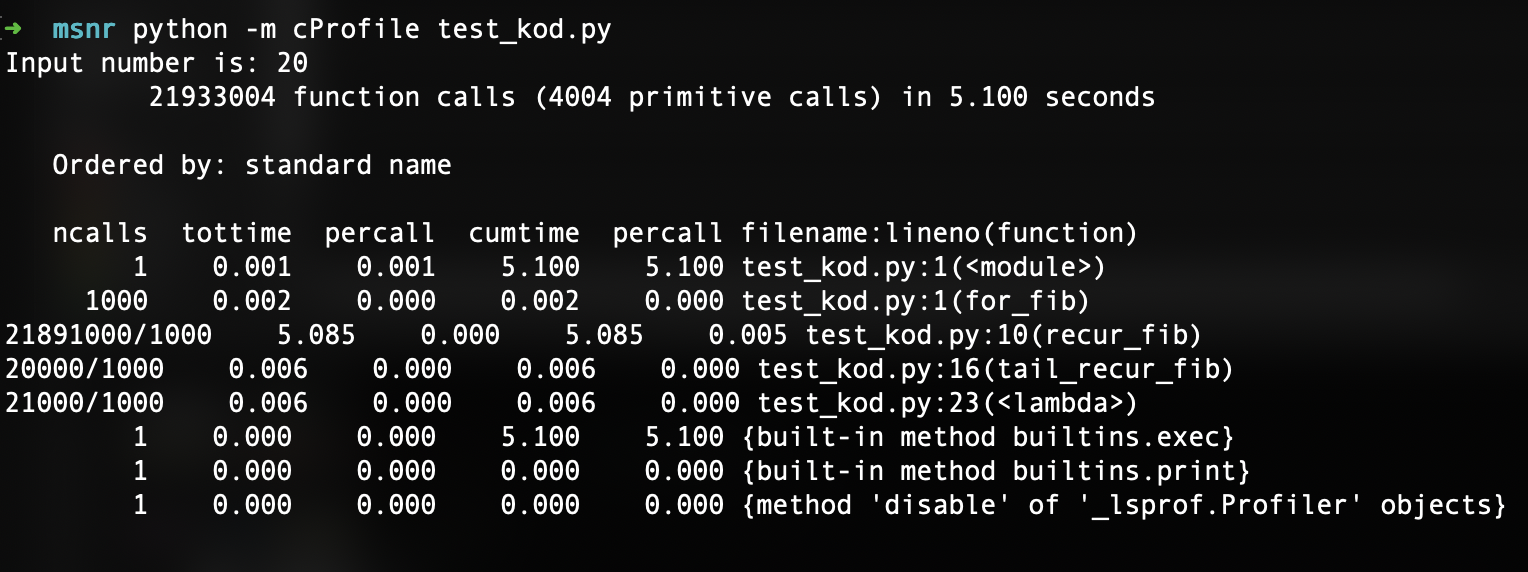
\includegraphics[scale=0.4]{MVJ_02_ProfajleriZaPython_ZecevicSmiljanicMilovanovicPopov/cProfile_without_import.png}
\end{center}
\caption{cProfile izveštaj}
\label{fig:ps_viz}
\end{figure}

\begin{center}
\scalebox{0.8}{\begin{minipage}{1.20\textwidth}
\begin{block}{primer pStats}
sortby = ’tottime’\\
ps = pstats.Stats(prof, stream=s).sort\_stats(sortby) 
\end{block}
\end{minipage}}
\end{center}
\end{frame}

\section{Alati za vizualizaciju profajliranja}
\begin{frame}{Alati za vizualizaciju profajliranja}
\begin{itemize}
\item Statistika koja se dobije profajliranjem je nečitljivija što je program kompleksniji
\item U cilju preglednosti, razvijeni su alati za vizualizaciju
\item Alati za vizualizaciju u Pythonu:
\begin{itemize}
\item Py-Spy
\item SnakeViz
\item Pycallgraph
\item gprof2dot
\item vprof
\end{itemize}
\end{itemize}
\end{frame}

\begin{frame}{Py-Spy}
\begin{figure}[h!]
\begin{center}
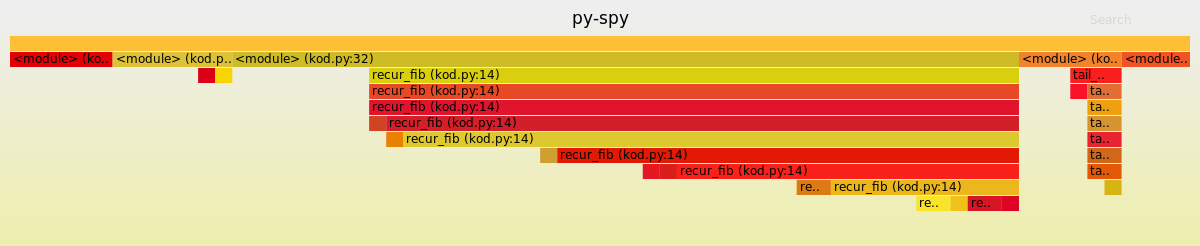
\includegraphics[scale=0.25]{MVJ_02_ProfajleriZaPython_ZecevicSmiljanicMilovanovicPopov/ps.png}
\end{center}
\caption{Py-Spy vizualizacija}
\label{fig:ps_viz}
\end{figure}
\end{frame}

\begin{frame}{SnakeViz}
\begin{figure}[h!]
\begin{center}
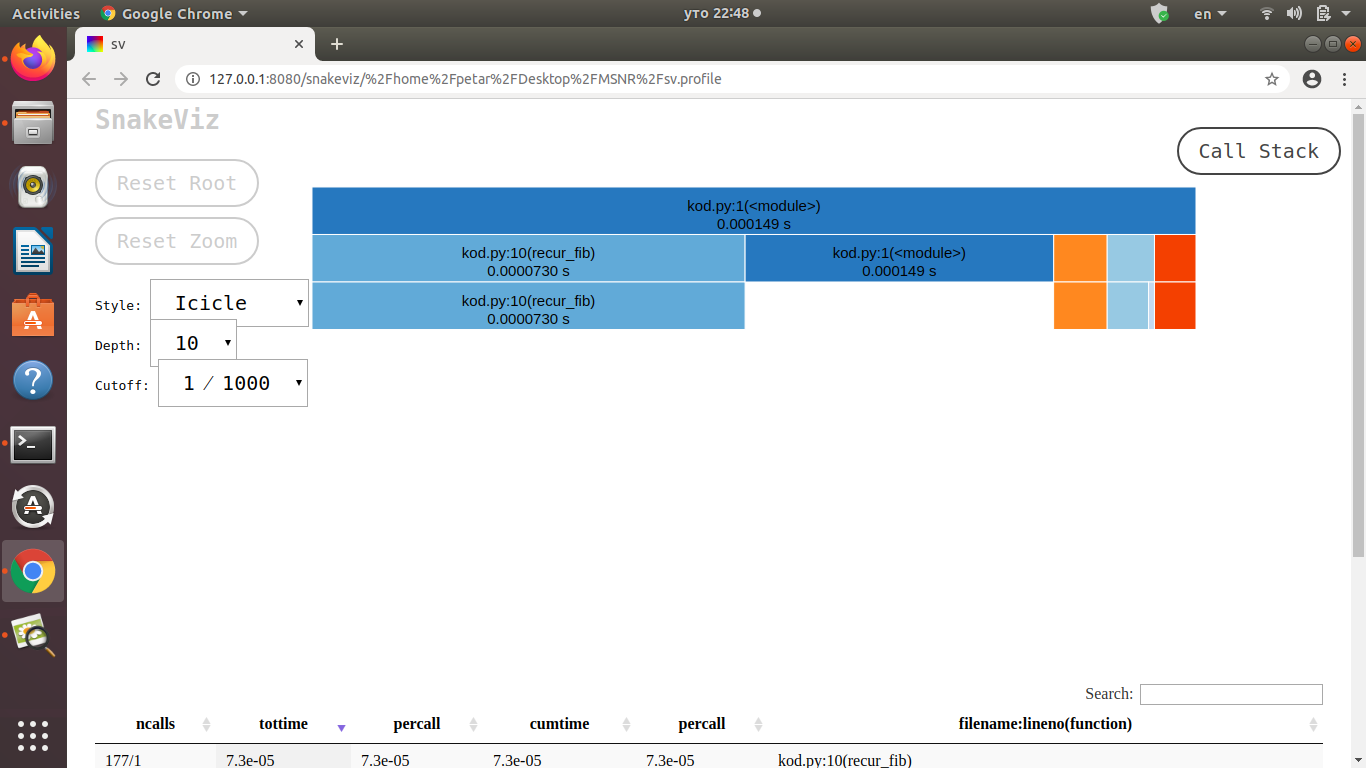
\includegraphics[trim={10cm 15cm 5cm 6.5cm},clip,scale=0.32]{snakeviz1.png}
\end{center}
\caption{SnakeViz vizualizacija}
\label{fig:snake_viz_1}
\end{figure}

\begin{figure}[h!]
\begin{center}
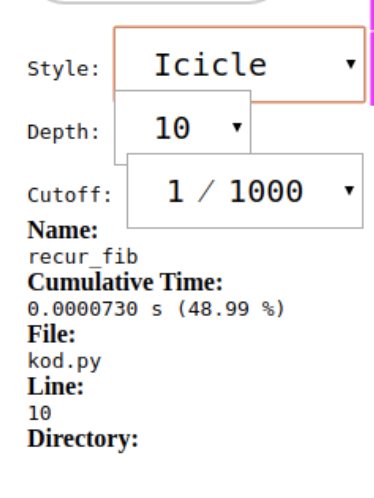
\includegraphics[trim={0cm 0cm 0cm 0cm},clip,scale=0.27]{snakeviz_statistic.png}
\end{center}
\caption{SnakeViz statistike}
\label{fig:snake_viz_2}
\end{figure}
\end{frame}

\begin{frame}{Pycallgraph}
\begin{figure}[h!]
\begin{center}
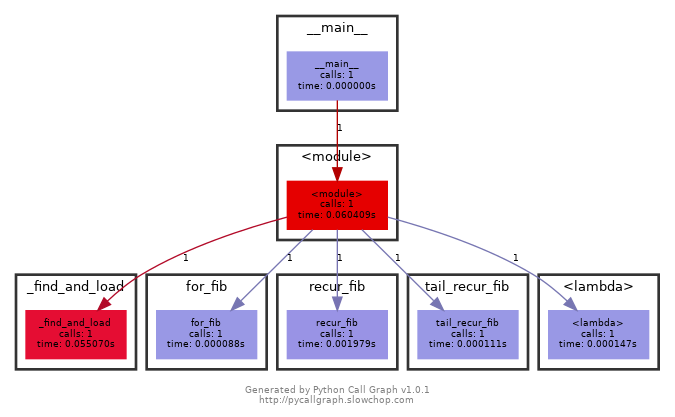
\includegraphics[scale=0.4]{pycallgraph.png}
\end{center}
\caption{Pycallgraph vizualizacija za graf dubine 2}
\label{fig:pycallgraph2_1}
\end{figure}
\end{frame}
 
\begin{frame}{Gprof2dot}
\begin{figure}[h!]
\begin{center}
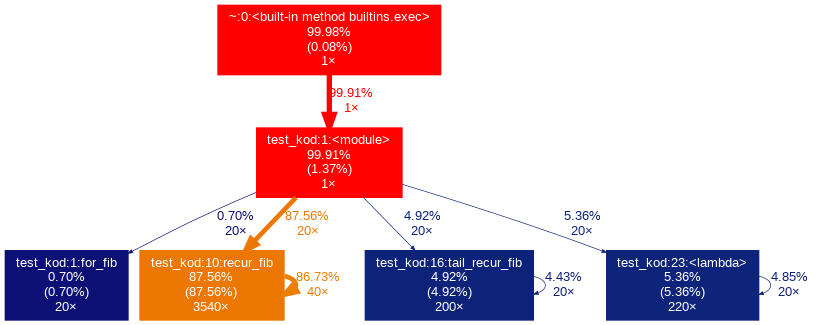
\includegraphics[scale=0.37]{MVJ_02_ProfajleriZaPython_ZecevicSmiljanicMilovanovicPopov/gprof2dot.png}
\end{center}
\caption{Gprof2dot vizualizacija}
\label{fig:gprof2dot_1}
\end{figure}
\end{frame}

\begin{frame}{Vprof}
\begin{figure}[h!]
\begin{center}
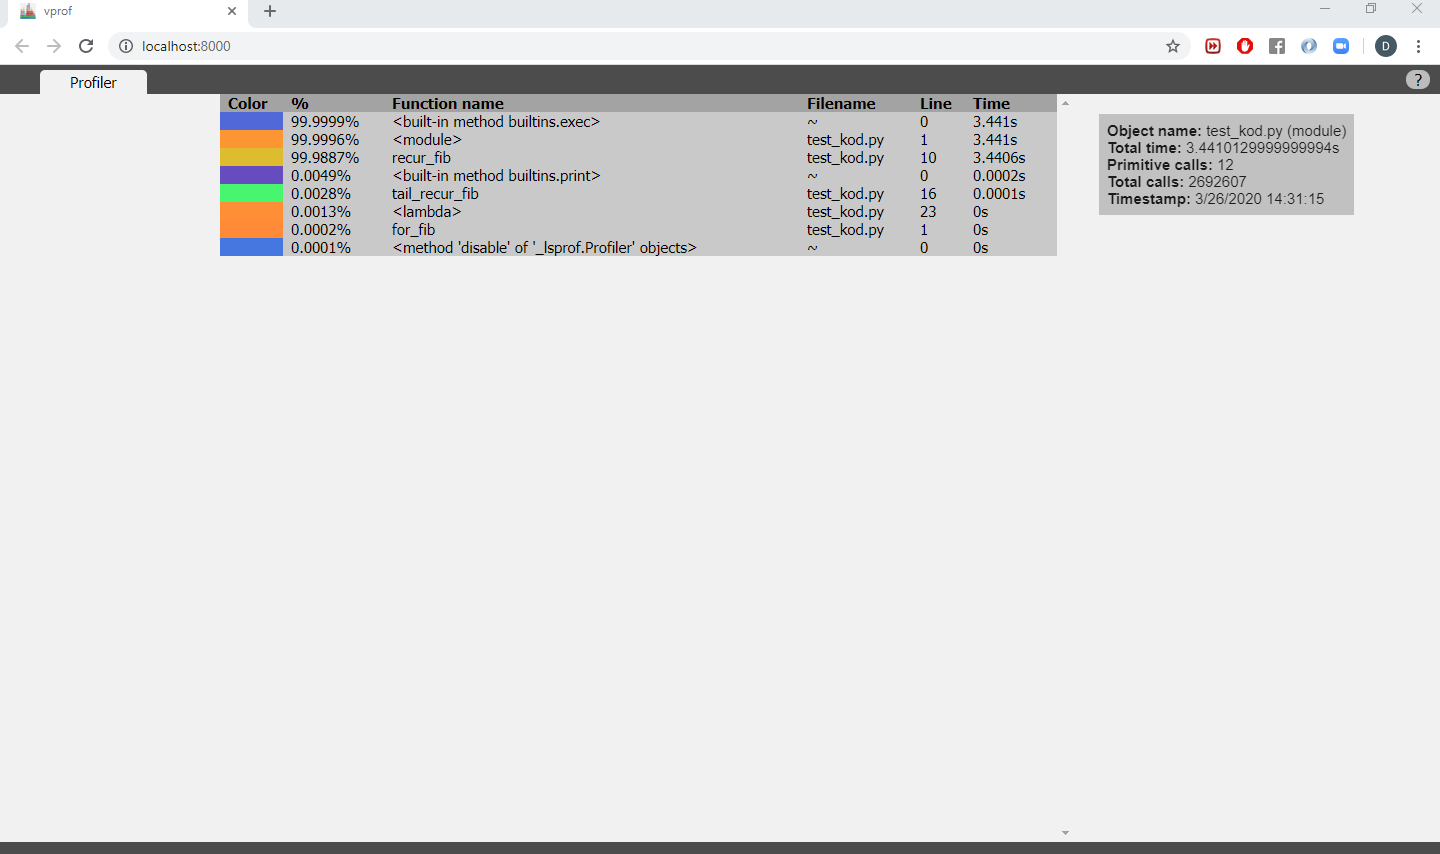
\includegraphics[trim={0cm 20cm 0cm 0cm},clip,scale=0.21]{MVJ_02_ProfajleriZaPython_ZecevicSmiljanicMilovanovicPopov/vprof.png}
\end{center}
\caption{Vprof vizualizacija}
\label{fig:vprof_1}
\end{figure}
\end{frame}

\section{Zaključak}
\begin{frame}{Zaključak}
\begin{itemize}
    \item Osnovne ideje vremenskog profajliranja
    \item Dobijanje jasnije slike o životu funkcija i izvršavanju celina koda
    \item Ubrzavanje procesa detekcije kritičnih delova koda
\end{itemize}
\end{frame}

\section{Literatura}
\begingroup
\setbeamertemplate{footline}{}
\begin{frame}{Literatura}
\scalebox{0.83}{\begin{minipage}{1.20\textwidth}
\bibliography{seminarski} 
\bibliographystyle{plain}
\nocite{opt}
\nocite{cProfile}
\nocite{lanaro2013python}
\nocite{profiling}
\end{minipage}}
\end{frame}
\endgroup
\end{document}